\section{Experimental methods and apparatus}\label{sec:experimental-technique-and-apparatus}
To examine the diffraction pattern from a helix we use the system described in Figure~\ref{fig:Apparatus}.
\begin{figure}[H]
    \centering
    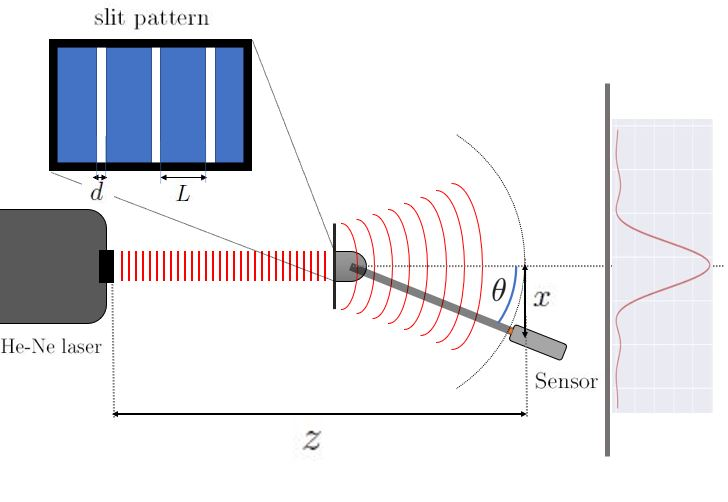
\includegraphics[width=0.9\columnwidth]{figures/Apparatus.JPG}
    \caption{A description of the system used to measure the intensity of light coming from a He-Ne laser at different angles. An example of a slit
    pattern is shown, but can be swapped for any diffracting object}
    \label{fig:Apparatus}
\end{figure}
Where the He-Ne laser produces an approximately monochromatic plane wave with $\lambda=632.8 [nm]$ and $z=1.9[m]\pm0.02[m]$
We also note that the sensor has an iris through which the light goes before measured, thus all light within that width is accounted for when measuring a
certain area on the screen.
For example the "Iris effect" in 1 dimension gives the expected intensity: $I(x)=\int\limits_{x-d}^{x+d}I(x')dx'$.
The sensor we used for measurement was a camera, and to analyse this diffraction pattern we take different sections of the photo and treat them as diffraction caused by different sections of the helix.
The camera we used not only has a 2-dimensional iris, but there's also the effect of "focus".
The camera's focus determines the distance for which a pixel describes the light that comes from the smallest area, simply put - distance of sharpest image.
Since our camera was placed at some angle relative to the laser beam, we measured diffraction at different distances from the camera and therefore could only achieve optimal focus for a single point of the diffraction pattern.
This suboptimal focus in the picture causes a similar effect to that of the iris in the sense that the intensity in every pixel is affected by the intensity of surrounding pixels.
